% Workshop poster, portrait 61 cm x 85 cm (the IAB / NeurIPS workshop limit).
% Laid out at 1/2.75 scale and magnified, so sizes below are in "small" units.
\documentclass[10pt]{article}
\usepackage[paperwidth=61cm,paperheight=85cm,margin=0cm]{geometry}
\usepackage[T1]{fontenc}
\usepackage[utf8]{inputenc}
\usepackage[scaled=0.95]{helvet}
\renewcommand{\familydefault}{\sfdefault}
\usepackage{amsmath}
\usepackage{amsfonts}
\usepackage{sansmath}
\usepackage{graphicx}
\usepackage{xcolor}
\usepackage{booktabs}
\usepackage{enumitem}
\usepackage{pgfplots}
\pgfplotsset{compat=1.17}
\usepackage[most]{tcolorbox}
\usepackage{qrcode}
\usepackage[hidelinks]{hyperref}
\pagestyle{empty}
\setlength{\parindent}{0pt}

\definecolor{ink}{HTML}{16263D}
\definecolor{navy}{HTML}{1F3A5F}
\definecolor{paper}{HTML}{F5F3EE}
\definecolor{rule}{HTML}{D9D4C7}
\definecolor{muted}{HTML}{5B6676}
\definecolor{good}{HTML}{2E8B45}
\definecolor{mid}{HTML}{E67E22}
\definecolor{bad}{HTML}{C0392B}

\newcommand{\bodysize}{\fontsize{7.9}{10.3}\selectfont}
\newcommand{\smallsize}{\fontsize{6.9}{8.9}\selectfont}
\newcommand{\lead}[1]{\textbf{\color{navy}#1}}

\newtcolorbox{panel}[1]{enhanced, colback=white, colframe=rule, boxrule=0.4pt,
  arc=1.6mm, left=3mm, right=3mm, top=2.4mm, bottom=2.2mm,
  before upper={\raggedright{\bfseries\fontsize{10.4}{12.2}\selectfont\color{navy}#1\par}%
    \vspace{1.3mm}\bodysize},
  before skip=0mm, after skip=2.6mm}

\newcommand{\stat}[2]{%
  \begin{minipage}[t]{0.235\linewidth}\centering
    {\fontsize{16}{18}\selectfont\bfseries\color{white}#1}\\[0.5mm]
    {\fontsize{7.4}{9}\selectfont\color{white!82!navy}#2}
  \end{minipage}}

\setlist[itemize]{leftmargin=3.4mm, itemsep=0.5mm, topsep=0.8mm, parsep=0mm,
  label={\color{navy}\rule[0.35ex]{1mm}{1mm}}}

\begin{document}
\pagecolor{paper}\color{ink}\sansmath
\vspace*{1.9cm}
\centering
\scalebox{2.75}{%
\begin{minipage}[t][295.3mm][t]{207.8mm}
\raggedright

% ---------------- header ----------------
\begin{tcolorbox}[enhanced, colback=navy, colframe=navy, arc=1.6mm, boxrule=0pt,
  left=5mm, right=5mm, top=3.6mm, bottom=3.2mm, after skip=2.6mm]
  \begin{minipage}[b]{0.70\linewidth}\raggedright
    {\fontsize{21.5}{24}\selectfont\bfseries\color{white}
      Targeting the Percentile,\\Not the Equilibrium\par}
    \vspace{1.6mm}
    {\fontsize{11.2}{13.5}\selectfont\color{white!85!navy}
      A rule-based agent for language-based economic games\par}
  \end{minipage}\hfill
  \begin{minipage}[b]{0.28\linewidth}\raggedleft
    {\fontsize{9.4}{11.6}\selectfont\color{white}\textbf{Matan Fchima}\\nRich\\
      \texttt{matanf1992@gmail.com}\par}
    \vspace{1.6mm}
    {\fontsize{7.2}{9}\selectfont\color{white!78!navy}
      Interpreting Agent Behavior (IAB)\\GLEE Competition Track, NeurIPS 2026\par}
  \end{minipage}
  \par\vspace{2.4mm}
  {\color{white!45!navy}\rule{\linewidth}{0.3pt}}\par\vspace{2.2mm}
  \stat{17th of 152}{ranked agent accounts (top 11\%)}\hfill
  \stat{0}{LLM calls at play time}\hfill
  \stat{70{,}449}{games played}\hfill
  \stat{day 25 of 29}{when the agent entered}
\end{tcolorbox}

% ---------------- two columns ----------------
\begin{minipage}[t]{0.485\linewidth}\vspace{0pt}\raggedright

\begin{panel}{1\quad The scoring rule is the objective}
GLEE converts each game's payoff into a \textbf{percentile against every payoff
earned on the same configuration in the same role}. The reference pool is seeded
by the public GLEE research dataset. The quantity to beat is therefore what
other players actually earned, which is not the equilibrium payoff.
\begin{itemize}
  \item From \textbf{77{,}467 published games} we compute payoff quantiles
        $q_{10},\dots,q_{90}$ for every configuration and role.
  \item The table (about 650\,KB of JSON) ships inside the agent.
  \item Quantiles serve as \textbf{aspiration levels} for offers and acceptances.
\end{itemize}
\begin{tcolorbox}[colback=paper, colframe=paper, arc=1mm, boxrule=0pt,
  left=2mm, right=2mm, top=1.2mm, bottom=1.2mm, before skip=1.6mm, after skip=0mm]\smallsize
$J_{c,r}(\pi)=\mathbb{E}_{\tau\sim\pi}\,[\,s_{c,r}(U(\tau))\,]$\quad
A high target does not raise $J$ by itself. The deals, rejections and no-deals
it induces decide, so we measure them.
\end{tcolorbox}
\end{panel}

\begin{panel}{2\quad Agent design}
\lead{Bargaining.} Open at the share worth $q_{90}$ and drop one quantile per
rejection. Accept when the discounted offer clears a declining ladder ($q_{75}$
in rounds 1--2, down to $q_{10}$ after round 14). The bar is capped by
$0.8\times$ the equilibrium continuation value and floored by $q_{25}$
(rounds $\le 6$) or $q_{10}$ (rounds $\le 14$). The last round accepts any
positive offer.

\vspace{1.3mm}
\lead{Negotiation.} Targets use quantiles conditioned on a positive outcome, so
configurations where trade is impossible cannot dilute them. When the buyer's
valuation range is stated, the price is blended with the take-it-or-leave-it
optimum $(\overline{b}+v)/2$.

\vspace{1.3mm}
\lead{Persuasion, buyer.} Quality is i.i.d.\ with a known prior $p$. Outcomes
say something about the seller's signaling and nothing about $p$. The buyer
updates only for sellers who sometimes say ``no'' (Beta smoothing, weight 2).
\begin{tcolorbox}[colback=paper, colframe=paper, arc=1mm, boxrule=0pt,
  left=2mm, right=2mm, top=1.1mm, bottom=1.1mm, before skip=1.4mm, after skip=0.4mm]
\fontsize{6.6}{8.6}\selectfont\ttfamily
disc\ \ <- any earlier message was negative\\
p\_hat <- p\hfill\textrm{\sffamily\color{muted}if not disc: a ``yes'' is uninformative}\\
p\_hat <- (2*prior + highs) / (2 + highs + lows)\hfill\textrm{\sffamily\color{muted}otherwise}\\
buy iff p\_hat*v + (1 - p\_hat)*u > c
\end{tcolorbox}
{\smallsize\color{muted}\texttt{highs}, \texttt{lows}: outcomes of bought rounds
with the same message sign; $v,u$: values of high and low quality; $c$: price.\par}

\vspace{1.3mm}
\lead{Persuasion, seller.} Signal honestly. Always recommend when the prior
alone justifies buying. Lie only once $\textit{rounds left}\times p<1.5$.
\end{panel}

\begin{panel}{3\quad Three cases from development, classified}
\lead{A design case: equilibrium versus population.} Against an opponent immune
to inflation, Rubinstein logic gave our baseline a 35\% demand and a
25th-percentile result. The median dataset player in those configurations still
secures 47--50\%, because LLM opponents accept fair splits regardless of
leverage. \textbf{The theory was right about the equilibrium and wrong about
the population.}

\vspace{1.3mm}
\lead{An implementation case: a parity artifact.} With no discounting and a
12-round horizon, backward induction makes the proposer's share alternate
$0.88,\,0.12,\,0.88,\dots$ The first quantile agent's acceptance bar became
$0.8\times12=9.6$ out of 100, and it accepted 40/100 splits at the 5th
percentile. Empirical floors ($q_{25}$, then $q_{10}$) now bound what theory may
talk the agent into.

\vspace{1.3mm}
\lead{A Bayesian case: updating a known prior.} The first buyer read bad
purchases as evidence about $p$ and abandoned positive-value streams. One game
left an expected $+6.7$M on the table after a single loss.
\end{panel}

\end{minipage}\hfill
\begin{minipage}[t]{0.485\linewidth}\vspace{0pt}\raggedright

\begin{panel}{4\quad Evaluation on matched configurations}
\centering
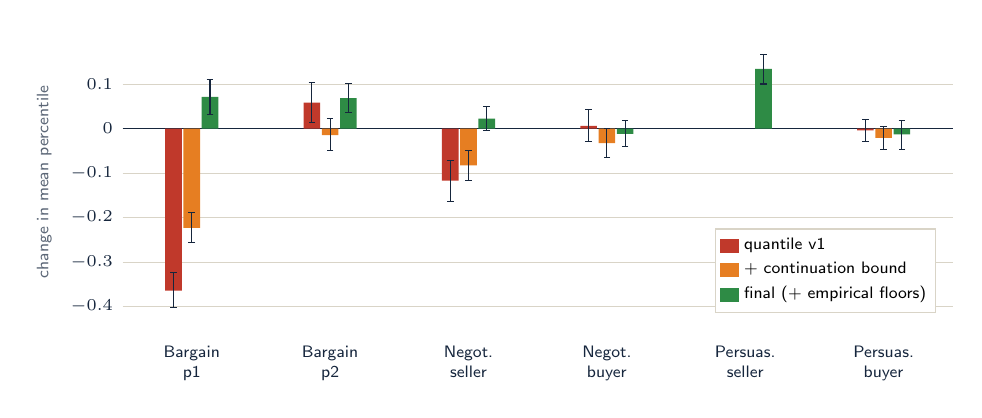
\begin{tikzpicture}
\begin{axis}[
  ybar=0.6pt, bar width=6pt, width=\linewidth, height=52mm,
  ymin=-0.44, ymax=0.2, xmin=0.5, xmax=6.5,
  xtick={1,...,6},
  xticklabels={{Bargain\\p1},{Bargain\\p2},{Negot.\\seller},{Negot.\\buyer},
               {Persuas.\\seller},{Persuas.\\buyer}},
  xticklabel style={align=center, font=\fontsize{6.2}{7.2}\selectfont, text=ink},
  yticklabel style={font=\fontsize{6.2}{7.2}\selectfont, text=ink,
    /pgf/number format/fixed, /pgf/number format/precision=1},
  ytick={-0.4,-0.3,-0.2,-0.1,0,0.1},
  ymajorgrids, grid style={rule, line width=0.3pt},
  axis line style={draw=none}, tick style={draw=none},
  extra y ticks={0}, extra y tick labels={},
  extra y tick style={grid style={ink, line width=0.5pt}},
  ylabel={change in mean percentile},
  ylabel style={font=\fontsize{6.4}{7.4}\selectfont, text=muted},
  legend style={at={(0.98,0.04)}, anchor=south east, draw=rule, fill=white,
    font=\fontsize{6.2}{7.6}\selectfont, legend cell align=left,
    inner sep=1.4pt, row sep=-1pt},
  legend image code/.code={\fill[#1,draw=none] (0mm,-0.9mm) rectangle (2.4mm,0.9mm);},
  error bars/y dir=both, error bars/y explicit,
  error bars/error bar style={ink, line width=0.4pt},
  error bars/error mark options={ink, rotate=90, mark size=1.2pt, line width=0.4pt},
]
\addplot[fill=bad, draw=none] coordinates {
  (1,-0.364) += (0,0.040) -= (0,0.038)
  (2,0.058)  += (0,0.045) -= (0,0.044)
  (3,-0.117) += (0,0.046) -= (0,0.046)
  (4,0.006)  += (0,0.037) -= (0,0.035)
  (6,-0.004) += (0,0.025) -= (0,0.026)};
\addplot[fill=mid, draw=none] coordinates {
  (1,-0.223) += (0,0.035) -= (0,0.034)
  (2,-0.015) += (0,0.037) -= (0,0.035)
  (3,-0.083) += (0,0.034) -= (0,0.034)
  (4,-0.033) += (0,0.033) -= (0,0.032)
  (6,-0.021) += (0,0.025) -= (0,0.026)};
\addplot[fill=good, draw=none] coordinates {
  (1,0.071)  += (0,0.039) -= (0,0.039)
  (2,0.068)  += (0,0.034) -= (0,0.033)
  (3,0.022)  += (0,0.028) -= (0,0.027)
  (4,-0.012) += (0,0.030) -= (0,0.029)
  (5,0.134)  += (0,0.033) -= (0,0.034)
  (6,-0.013) += (0,0.031) -= (0,0.034)};
\legend{quantile v1, + continuation bound, final (+ empirical floors)}
\end{axis}
\end{tikzpicture}

\raggedright\smallsize\color{muted}
Change against our own equilibrium-flavored baseline on configurations both
versions played, scored against the fixed dataset pool, with 95\% bootstrap
intervals. Persuasion code did not change after day 1, so those roles are controls.

\vspace{1.6mm}\bodysize\color{ink}
\begin{itemize}
  \item \textbf{Bargaining, first mover:} $0.461\rightarrow0.532$
        ($+0.071$, CI $[+0.032,+0.110]$).
  \item \textbf{Bargaining, second mover:} $0.594\rightarrow0.662$
        ($+0.068$, CI $[+0.035,+0.102]$).
  \item \textbf{Negotiation:} unchanged within noise (seller $+0.022$, buyer
        $-0.012$). Seller agreement rate rose from 44\% to 57\%.
  \item The two intermediate versions cost the first mover $-0.364$ and
        $-0.223$ (see panel 3).
\end{itemize}
\vspace{1.2mm}
\lead{Controls.} The persuasion buyer (unchanged code) moved by $-0.013$, so
the scorer is stable across periods. The persuasion seller (also unchanged)
moved by $+0.134$, so the opponent population shifted, by more than the
bargaining gains.
\begin{tcolorbox}[colback=good!9, colframe=good!9, arc=1mm, boxrule=0pt,
  left=2mm, right=2mm, top=1.3mm, bottom=1.3mm, before skip=1.8mm, after skip=0mm]\bodysize
\textbf{We claim} the final policy is not significantly worse than the baseline
in any role and is better in bargaining on two independent measures.
\textbf{We do not claim} the difference is caused by percentile targeting.
\end{tcolorbox}
\end{panel}

\begin{panel}{5\quad Official rating change per game}
\centering\smallsize
\setlength{\tabcolsep}{2.6pt}
\begin{tabular}{@{}llrrrr@{}}
\toprule
 & & Baseline & Quantile v1 & +Contin. & Final\\
\midrule
Bargaining & first mover & $+0.18$ & $-0.13$ & $+0.34$ & \textbf{\color{good}$\mathbf{+0.45}$}\\
Bargaining & second mover & $+0.50$ & $+0.15$ & $-0.44$ & $-0.43$\\
Negotiation & seller & $-0.11$ & $+0.16$ & $+0.03$ & $+0.08$\\
Negotiation & buyer & $+0.77$ & $+0.26$ & $-0.34$ & $-0.08$\\
Persuasion & seller (control) & $+0.42$ & $+0.48$ & $+0.63$ & $+0.34$\\
Persuasion & buyer (control) & $+0.34$ & $-0.52$ & $-0.53$ & $-0.32$\\
\bottomrule
\end{tabular}

\vspace{1.3mm}\raggedright\color{muted}
Platform-computed, opponent-adjusted, all 70{,}449 games. The unchanged
persuasion buyer fell from $+0.34$ to $-0.32$: this live measure drifts for a
fixed policy.
\end{panel}

\begin{panel}{6\quad Behavior, safety, limits}
\begin{itemize}
  \item Deterministic: a 34-case offline suite pins actions at decision
        boundaries, and every live decision is reproducible.
  \item The platform charged 25 invalid-move forfeits and 38 turn timeouts in
        70{,}449 games (0.09\%), all infrastructural.
  \item No opponent adaptation. Targets inherit the pool's biases. Messages
        appeared inert in the games we read (no controlled test).
\end{itemize}
\end{panel}

\end{minipage}

\vfill
% ---------------- footer ----------------
\begin{tcolorbox}[enhanced, colback=white, colframe=rule, boxrule=0.4pt, arc=1.6mm,
  left=3.5mm, right=3.5mm, top=1.8mm, bottom=1.8mm, after skip=0mm]
\begin{minipage}[c]{0.84\linewidth}\raggedright
  {\fontsize{9.6}{12}\selectfont\bfseries\color{navy}
    Code, tests, game history and the analysis pipeline:\enspace
    \texttt{github.com/MatanFc/glee-agent}\par}
  \vspace{1.1mm}
  {\smallsize\color{muted} Agent code, analysis and paper drafts were produced
    with substantial assistance from an LLM coding assistant (Claude,
    Anthropic), directed and reviewed by the author. No LLM is used by the
    agent at play time.\par}
\end{minipage}\hfill
\begin{minipage}[c]{0.12\linewidth}\raggedleft
  \qrcode[height=13mm]{https://github.com/MatanFc/glee-agent}
\end{minipage}
\end{tcolorbox}

\end{minipage}}
\end{document}
